\subsubsection*{(一) 量測方式}
\begin{enumerate}
    \item 架設暗室以阻隔環境光，將裝有樣品的方形比色槽放在以雙面膠標示的固定位置。
    \item 調整旋轉臂角度與高度，使直射光剛好照到感測器，並以此位置定為 $0^\circ$。比色槽面向雷射，使槽壁大致垂直於雷射光、但略向前傾，避免反射光直接返回雷射而影響輸出。
    \item 關閉雷射，量測暗室背景與暗讀值；暗室環境亮度確認低於 $0.001\,\mathrm{lux}$。
    \item 開啟雷射後，旋轉臂每次轉動 $1^\circ$ 並停留約 $2$ 秒；含馬達與程式執行時間，每格實測週期約 $2.45$ 秒。旋轉臂由 $0^\circ$ 量至 $140^\circ$ 後返回原位，為一輪；每個樣品量測兩輪，約需 $12$ 分鐘。
    \item 回到 $0^\circ$ 時比對初始讀值，以確認旋轉臂是否回到原位。依 Stokes 定律估算，$2.16\,\mu\mathrm{m}$ 微球在水中的沉降速度約 $0.5\,\mathrm{mm/h}$，一次量測期間沉降約 $0.1\,\mathrm{mm}$，可忽略。
\end{enumerate}
\begin{figure}[H]
    \centering
    % 左邊的照片（寬度設為版面的 48%）
    \begin{subfigure}[b]{0.48\textwidth}
        \centering
        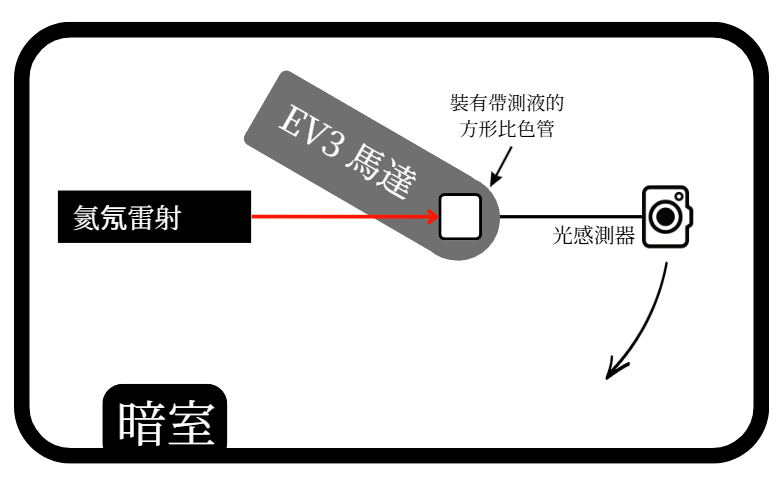
\includegraphics[width=\textwidth]{image/structure.png}
        \caption{裝置實照}\label{fig:left}
    \end{subfigure}
    \hfill 
    \begin{subfigure}[b]{0.48\textwidth}
        \centering
        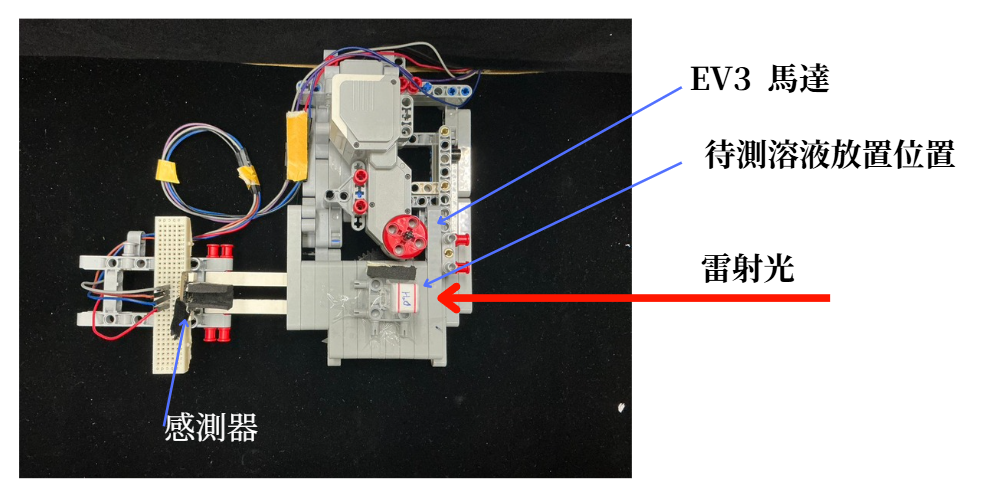
\includegraphics[width=\textwidth]{image/structure_image.png}
        \caption{裝置示意圖}\label{fig:right}
    \end{subfigure}\label{fig:both}
\end{figure}

\subsubsection*{(二) 感測器增益與空白量測}
感測器增益與積分時間由韌體依讀值切換：預設為 HIGH 增益、積分時間 $600\,\mathrm{ms}$；全光譜通道 CH0 低於 $5000$ 時，切換至 MAX 增益、$200\,\mathrm{ms}$，並維持至 CH0 超過 $50000$ 或飽和後才切回 HIGH，以減少頻繁切換。若 HIGH 飽和，則改以 MED 增益、$100\,\mathrm{ms}$ 補讀一筆，該筆不納入分析。依規格書，HIGH 與 MAX 的典型增益分別約為 LOW 的 $400$ 倍與 $9200$ 倍；同型晶片的 HIGH 增益範圍約為 $360$ 至 $440$ 倍，MAX 約為 $8500$ 至 $9900$ 倍（ams-OSRAM AG, 2023）。量測當天於不同時段各量一次純水空白，並量測雷射關閉時的暗讀值。

\subsubsection*{(三) 數據監測方式}
以 Rust 撰寫監測程式，持續讀取 Arduino 的序列埠資料並存成 CSV，以供後續處理。

\subsubsection*{(四) 數據處理}
\begin{enumerate}
    \item 僅保留完整讀值列；剔除飽和讀值、增益切換後的第一筆，以及偏離中位數超過 $4$ 倍穩健標準差的離群值。
    \item 依實測步進週期 $2.45$ 秒推算每個角度格的時間區間，只保留整段曝光都發生在旋轉臂靜止期間的讀值，每格取中位數。
    \item 由每格時間推定臂角（每格 $1^\circ$），再依當天記錄修正角度零點。
    \item 將 HIGH 讀值乘以倍率 $r$，換算為 MAX 等效讀值。依兩種設定的典型增益與積分時間估算，$r=(9200/400)\times(200/600)\approx7.7$；考量晶片個體差異，以旋轉臂靜止且同一格同時有兩種增益讀值的位置，取 MAX 與 HIGH 中位數之比實測，得到 $r=7.48$。此值落在規格範圍內；$30^\circ$ 與 $125^\circ$ 均以 MAX 量得，因此 $C$ 不受此換算影響。
    \item 扣除第二次量測的純水空白，計算淨強度
    \[
        I_{\mathrm{net}}(\theta)=I_{\mathrm{sample}}(\theta)-I_{\mathrm{blank}}(\theta).
    \]
    \item 每輪分別計算 $C=I_{\mathrm{net}}(30^\circ)/I_{\mathrm{net}}(125^\circ)$，再取兩輪平均。
    \item 不確定度取三項平方和開根號：兩輪 $C$ 差的一半、改用另一次純水空白所造成差異的一半，以及角度整體偏移 $\pm0.5^\circ$ 所造成差異的一半。
\end{enumerate}